\documentclass[12pt]{article}

\usepackage{sbc-template}

\usepackage{graphicx,url}

\usepackage[brazil]{babel}   
%\usepackage[latin1]{inputenc}  
\usepackage[utf8]{inputenc}  
% UTF-8 encoding is recommended by ShareLaTex

     
\sloppy

\title{Review: Handover Implementation in a 5G SDN-based Mobile Network Architecture}

\author{Antônio O. Junior\inst{1}, Cleverson V. Nahum\inst{1}, Felipe H. B. Bastos\inst{1}, Jamelly F. Ferreira\inst{1}, \\João C. Belmiro\inst{1} }


\address{Faculdade de Engenharia da Computação e Telecomunicações \\-- Universidade Federal do Pará
  (UFPA)\\
  Caixa Postal 479 -- 66.075-110 -- Belém -- PA -- Brazil
  \email{\{antonio,jamelly,felipe,joao\}@itec.ufpa.br, cleversonahum@ufpa.br}
}

\begin{document} 

\maketitle

\begin{abstract}
  This meta-paper describes the style to be used in articles and short papers
  for SBC conferences. For papers in English, you should add just an abstract
  while for the papers in Portuguese, we also ask for an abstract in
  Portuguese (``resumo''). In both cases, abstracts should not have more than
  10 lines and must be in the first page of the paper.
\end{abstract}
     
\begin{resumo} 
  Este meta-artigo descreve o estilo a ser usado na confecção de artigos e
  resumos de artigos para publicação nos anais das conferências organizadas
  pela SBC. É solicitada a escrita de resumo e abstract apenas para os artigos
  escritos em português. Artigos em inglês deverão apresentar apenas abstract.
  Nos dois casos, o autor deve tomar cuidado para que o resumo (e o abstract)
  não ultrapassem 10 linhas cada, sendo que ambos devem estar na primeira
  página do artigo.
\end{resumo}


\section{Introduction}

All full papers and posters (short papers) submitted to some SBC conference,
including any supporting documents, should be written in English or in
Portuguese. The format paper should be A4 with single column, 3.5 cm for upper
margin, 2.5 cm for bottom margin and 3.0 cm for lateral margins, without
headers or footers. The main font must be Times, 12 point nominal size, with 6
points of space before each paragraph. Page numbers must be suppressed.

Full papers must respect the page limits defined by the conference.
Conferences that publish just abstracts ask for \textbf{one}-page texts.

\section{Background} \label{sec:sdn}
\subsection{SDN}

The SDN (Software-Defined Networking) is a recently concept of network, nowadays the most part of the networks has a distributed control in the their elements. So, with the growth of the multimedia and the increases of flows of data traffic in the world, it emerged necessity to have more control over the network and more mobility in the chooses, the networks need to be more flexible. With this need the SDN was thought to solve some problems in the actual architecture.

The main of SDN is split the data plane (data flow) of control plane (control flow) and centralized all the control of the network in a unique place named Controller. In the SDN, it has a division between APPs, control plane and data plane, it is possible to seen in the picture N. The APPs are applications with functions related to security, network management and others, they are responsible to make security and other needs of the network, in the traditional architecture this responsible is distributed in the elements of network, how SDN has more informations about the network, it became more easy to make decisions about the flow paths, to solve congestions and other problems faced in networks.

The control plane is represented by the Controllers, it is responsible to control the switches OpenFlow in according with algorithms and configurations established in APPs. The communication between Controllers and APPs is done through northbound interface. With the Controllers is possible to set all the connections of the switch through software. The OpenFlow switch quoted is a special switch made for to work with SDN networks.

The data plane is represented by the switches, OpenFlow switches is the principal, The communication between Controllers and switches is done through southbound interface. The OpenFlow switches is more simple than traditional switches and its communication and iteration is made through a API. In the traditional switches we have a proprietor systems for each one, it became more complex to implement a network because the systems is much specifically. With the switches OpenFlow the work of switches is more simple and it can be more flexible, because now all the connections can be defined in the software, moreover, it has more freedom to make changes in its, because of the iteration level is higher than traditional switches.

Picture N

In the actual architecture, it has the data plane and control plane distributed on the routers, servers, clients ans other elements of the network, with this all the control of network became more complex and hard to manage. The SDN proposed a different way of see the network, it allow to centralize the control of network in a place, with is, it is possible to see all the nodes and connections of the network and to know about everything that occurs, thereby it is possible to do the better actions for to improve the network performance. The figure N2 shows a illustrations of the difference between the networks in a traditional architecture, in a hybrid and using SDN. In a traditional networking, there is the data plane and control plane in all the components of the network, it is distributed. In hybrid networking there is a controller over the traditional networking for to control the switches and elements of the network. In the SDN, there is a clear division between data plane and control plane, the switches has only the data planes and the controller has the control plane.


The first page must display the paper title, the name and address of the
authors, the abstract in English and ``resumo'' in Portuguese (``resumos'' are
required only for papers written in Portuguese). The title must be centered
over the whole page, in 16 point boldface font and with 12 points of space
before itself. Author names must be centered in 12 point font, bold, all of
them disposed in the same line, separated by commas and with 12 points of
space after the title. Addresses must be centered in 12 point font, also with
12 points of space after the authors' names. E-mail addresses should be
written using font Courier New, 10 point nominal size, with 6 points of space
before and 6 points of space after.

The abstract and ``resumo'' (if is the case) must be in 12 point Times font,
indented 0.8cm on both sides. The word \textbf{Abstract} and \textbf{Resumo},
should be written in boldface and must precede the text.

\section{5G and Mobility}

In some conferences, the papers are published on CD-ROM while only the
abstract is published in the printed Proceedings. In this case, authors are
invited to prepare two final versions of the paper. One, complete, to be
published on the CD and the other, containing only the first page, with
abstract and ``resumo'' (for papers in Portuguese).

\section{Related Works}

Section titles must be in boldface, 13pt, flush left. There should be an extra
12 pt of space before each title. Section numbering is optional. The first
paragraph of each section should not be indented, while the first lines of
subsequent paragraphs should be indented by 1.27 cm.

\subsection{Subsections}

The subsection titles must be in boldface, 12pt, flush left.

\section{System Architecture}

Section titles must be in boldface, 13pt, flush left. There should be an extra
12 pt of space before each title. Section numbering is optional. The first
paragraph of each section should not be indented, while the first lines of
subsequent paragraphs should be indented by 1.27 cm.

\section{Handover Procedure}

Section titles must be in boldface, 13pt, flush left. There should be an extra
12 pt of space before each title. Section numbering is optional. The first
paragraph of each section should not be indented, while the first lines of
subsequent paragraphs should be indented by 1.27 cm.

\section{SDN-Based Mobility Support}

Section titles must be in boldface, 13pt, flush left. There should be an extra
12 pt of space before each title. Section numbering is optional. The first
paragraph of each section should not be indented, while the first lines of
subsequent paragraphs should be indented by 1.27 cm.

\section{Results and discussions}

Section titles must be in boldface, 13pt, flush left. There should be an extra
12 pt of space before each title. Section numbering is optional. The first
paragraph of each section should not be indented, while the first lines of
subsequent paragraphs should be indented by 1.27 cm.

\section{Conclusions}

Section titles must be in boldface, 13pt, flush left. There should be an extra
12 pt of space before each title. Section numbering is optional. The first
paragraph of each section should not be indented, while the first lines of
subsequent paragraphs should be indented by 1.27 cm.

\section{Figures and Captions}\label{sec:figs}


Figure and table captions should be centered if less than one line
(Figure~\ref{fig:exampleFig1}), otherwise justified and indented by 0.8cm on
both margins, as shown in Figure~\ref{fig:exampleFig2}. The caption font must
be Helvetica, 10 point, boldface, with 6 points of space before and after each
caption.

\begin{figure}[ht]
\centering
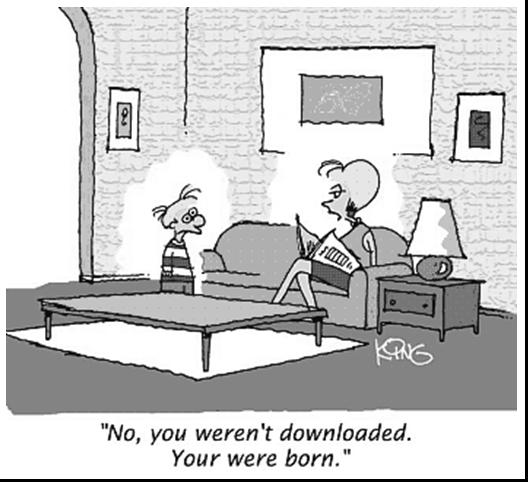
\includegraphics[width=.5\textwidth]{fig1.jpg}
\caption{A typical figure}
\label{fig:exampleFig1}
\end{figure}

\begin{figure}[ht]
\centering
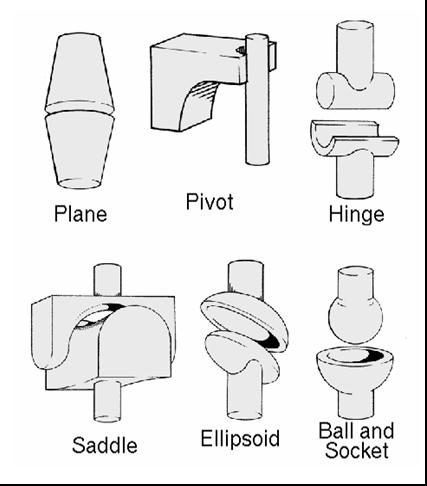
\includegraphics[width=.3\textwidth]{fig2.jpg}
\caption{This figure is an example of a figure caption taking more than one
  line and justified considering margins mentioned in Section~\ref{sec:figs}.}
\label{fig:exampleFig2}
\end{figure}

In tables, try to avoid the use of colored or shaded backgrounds, and avoid
thick, doubled, or unnecessary framing lines. When reporting empirical data,
do not use more decimal digits than warranted by their precision and
reproducibility. Table caption must be placed before the table (see Table 1)
and the font used must also be Helvetica, 10 point, boldface, with 6 points of
space before and after each caption.

\begin{table}[ht]
\centering
\caption{Variables to be considered on the evaluation of interaction
  techniques}
\label{tab:exTable1}
\smallskip
\begin{tabular}{|l|c|c|}
\hline
& Value 1 & Value 2\\[0.5ex]
\hline
&&\\[-2ex]
Case 1 & 1.0 $\pm$ 0.1 & 1.75$\times$10$^{-5}$ $\pm$ 5$\times$10$^{-7}$\\[0.5ex]
\hline
&&\\[-2ex]
Case 2 & 0.003(1) & 100.0\\[0.5ex]
\hline
\end{tabular}
\end{table}

\section{Images}

All images and illustrations should be in black-and-white, or gray tones,
excepting for the papers that will be electronically available (on CD-ROMs,
internet, etc.). The image resolution on paper should be about 600 dpi for
black-and-white images, and 150-300 dpi for grayscale images.  Do not include
images with excessive resolution, as they may take hours to print, without any
visible difference in the result. 

\section{References}

Bibliographic references must be unambiguous and uniform.  We recommend giving
the author names references in brackets, e.g. \cite{knuth:84},
\cite{boulic:91}, and \cite{smith:99}.

The references must be listed using 12 point font size, with 6 points of space
before each reference. The first line of each reference should not be
indented, while the subsequent should be indented by 0.5 cm.

\bibliographystyle{sbc}
\bibliography{sbc-template}

\end{document}
